\PassOptionsToPackage{table}{xcolor}

\documentclass[sigchi]{acmart}
\usepackage[utf8]{inputenc}
\usepackage{booktabs}
\usepackage{array}
\usepackage{tabularx}
\usepackage{balance}

\graphicspath{ {./figures/} }


\title[Transmodal News Behavior]{Transmodal News Behavior: Exploring How People Curate and Manage Their News Consumption}
\date{May 4, 2019}

%Conference
\acmConference[CHI 2019]{CHI 2019}{May 2019}{Glasgow, UK}

%\setcopyright{none} 
\begin{document}
\raggedbottom


\author{Second Author}
\affiliation{Affiliation}
\city{test 1}
\country{Country}
\email{e-mail address}

\author{First Author}
\affiliation{Affiliation}
\city{City}
\country{Country}
\email{e-mail address}
  



\begin{abstract}
The disruption of the news industry has forced us all to be the designers and curators of our own news and information ecosystems. Using what we call a transmodal approach, we conducted a two-week diary study with 14 participants to observe how news users fluidly switch between different media, sources, platforms and devices. This approach opened up a deeper understanding of the motivations and values underlying news behaviors than would have been possible by studying any single news platform alone. We found that people frequently shift their focus between ambient background news streams and foreground news content. Although news backgrounding is a passive activity, people actively manage background news habits to increase the chances of relevant foreground experiences. We encourage new product designers to consider these implications: treat backgrounding as an essential part of news consumption behavior, leverage the awareness self-tracking produces, and acknowledge the social currency of news.
\end{abstract}

\keywords{News, media consumption, multitasking, cross-platform, cross-media, diary study, transmodal, passive media}

\settopmatter{printfolios=true}

\maketitle

\section{Introduction}
The changing media technology landscape has thrown the news industry into upheaval. Daily U.S. newspaper circulation continues to decline year over year, as does their key revenue stream, advertising\cite{pewnewspapers}.\cite{pew} Simultaneously, the ubiquity of mobile devices, the abundance of digital news outlets, and the growing role of social media are changing how people find news content. As content is dispersed in new ways, traditional news media categories (such print and broadcast media) have merged with digital experiences, blurring the boundaries between these categories. Faced with media convergence and diffuse news content, individuals are now cast as the (sometimes accidental) designers and curators of their own personal news and information ecosystems.

 Nine-in-ten U.S. adults consume news content online\cite{pew_stocking_2018}, but news behavior is far from homogeneous. People engage in, and switch between, different \textit{behavioral modes}—reading, listening, or watching—while consuming news content. However, these behavioral modes are inseparable from other news consumption modalities—media, platform, device, and source. With \emph{cross-media} modality, users can quickly switch between text-, video-, and audio-based experiences. They can also move \emph{cross-platform}, switching between distribution methods like news websites or podcasting apps, or \emph{cross-device} switching between smartphones, computers, TVs, radios, and smart speakers. Finally, users can move \emph{cross-source} as they encounter content via word of mouth, social media, news aggregators, and traditional news outlets. 
 
It's important to understand news behaviors in order to better foster civic engagement within communities; Ksiaszek, Malthouse, and Webster\cite{ksiazek2010news} showed a positive relationship between news consumption and civic participation such as being part of in civically driven community organizations. Yes these increasingly individualized, multi-dimensional, self-curated news behaviors are difficult to study. Past research in New Media Studies has looked at news consumption [TKTKTK]. HCI has explored  social interactions with news \cite{Lottridge:2018:LHT:3173574.3173634}, but consumption research has often focused on single-platform analysis such as news on Facebook [citation] or Reddit \cite{Leavitt:2014:UHS:2556288.2557140}\cite{ Leavitt:2017:UMN:3171581.3134700}. Driscoll and Thorson \cite{driscoll2015searching}  critique these single-platform approaches to studying news behaviors because they can't capture the richness of people's lived experiences. Instead, they advocate for cross-platform approach. To understand how news platforms fit into the larger context of how people are engaging with news, we need to understand motivations, intents, and catalysts for news engagement. 

The goal of our research is to understand the attitudes and values underlying people’s news consumption preferences and behaviors holistically, across media types and technology platforms, in order to guide the development of future news media products to meet people’s information needs. We set out to look at the holistic ways people interact with news in their daily routines. Specifically, we ask the following research questions:
\begin{enumerate}
    \item Why do people choose between reading, listening, and watching their news content?
    \item How do situational contexts drive news consumers to seek out and switch between news modes?
    \item How do routines, habits, and social context influence consumption of (or abstinence from) news?
\end{enumerate}

To address these questions, we conducted a two-week diary study with 14 individuals across the U.S. who frequently consume news content. There are widely varying definitions of what makes content newsworthy \cite{harcup2001news}. We adopt Lee's \cite{lee2013news} universal approach to news which includes both "harder" and "softer" genres. Hard news is typically related to current events, whereas soft news stories are not time-specific and more likely to be of human interest \cite{tuchman1973making}. We allowed our participants to self-define news without imposing any genre constraints, which means our study includes entertainment, sports and special interest news topics. 

Our study, built and designed upon a phenomenological approach \cite{smith_flowers_larkin_2013}, began with an introductory interview, followed by 11 days of remote participant tracking and logging through an online blogging platform and daily voicemails. We concluded the diary study with an hour-long interview. We analyzed our qualitative data through an iterative and inductive affinity diagramming technique. This data and analysis sheds new light on how people navigate news using both background and foreground attention, and how they curate, manage, and consume news across media and platforms. It also reveals the social currency of how news is used in interactions with others, and the implications of self-tracking news behaviors. 

This paper contributes to a deeper understanding of the way in which digital experiences mediate news consumption for users by introducing a \textit{transmodal news consumption} framework. We show how news is both an individual and a collective experience that transitions between the digital and analog world. We also present design implications for treating backgrounding as an essential part of news consumption behavior, leveraging the awareness self-tracking produces, and acknowledging the social currency of news. This is important for designing platforms related to how people consume news-related content - whether that is through social media, apps, voice interactions,and or other digital content distribution platforms.

\section{Related Work}
Research on news consumption behavior sits at the intersection of media studies, journalism, political sciences, and technology studies. In this section, we present a cross-disciplinary look at work related to our research questions. 

\subsection{The state of the news}
Pew Research Center tracks trends and patterns in the media and news landscape. As of 2017, 50 percent of American adults "often" get news from TV, 43 percent from online sources, 25 percent from radio, and 18 percent from print newspapers. \cite{pew_TVonline} Recent survey reports from this group show that 68 percent of Americans "at least occasionally" get news from social media; Reddit, Twitter, and Facebook are the most popular. But 57 percent of Americans distrust social media and consider it to be an inaccurate news source. \cite{pew_newsusesocial2018}

\subsection{Media Repertoires and Uses and Gratifications as ways to understand news choices}
A Media Repertoire, or the subset of available media choices that an individual regularly uses, is a commonly used framework in understanding how individuals integrate multiple media choices to form. 

Audience centered - use and gratification
Media centered - structural
Yuan - repertoire 
Webster Duality 

Yuan \cite{yuan2011news} proposed a repertoire approach to looking at news consumption across multiple media platforms and found user's interest in and the availability of news impacts the size of a person's repertoire - investigating both structural and agency centered factors in peoples news repertoires. 
Similarly Webster \cite{webster2011duality} proposed a combination of individual and structural factors into a single model around the duality of media. where both individual preferences an gratifications are constrained an impacted by media availability. 

Between these frameworks, it's clear that a mix of both individual and structural factors impact how users create their media and news repertoires. However, little work has been done to understand how users navigate their repertoires by looking at platforms, devices, sources, and media types together. 



----
Scratch Pad
New media and technology studies focused on news often draw on the uses and gratifications framework for understanding news consumption behaviors. The two  The Uses and Gratification approach emphasizes an individual or audiences' role in how media is selected and used. It assumes that media content is driven by individual needs rather than [find the paper that has the differences between audience and content centered approaches.]

The Uses and Gratifications approach centers around how individual predispositions, such as preferences, needs, or psychological states, influence a person's choices around media consumption. It leverages principles such as 1) audiences are active consumers of media content, 2) people use media to satisfied certain needs, 3)media use is driven by a variety of motivations and 

---
\subsection{Transmodal Section: Sources, Platforms, Modes, and Media}
a section of stuff goes here
This could be useful: "When News is Everywhere" (advocates for a "radical user perspective on journalism" but doesn't go as far as to use diary studies)
\subsection{Multitasking and context of news consumption}
a section of stuff goes here. Look at Danielle and Mia's paper on multitasking and live streaming. 
\subsection{Digital news and CHI}
a section of stuff goes here 
 - social sharing 
 - specific events
 - social media 

This related work shows how media studies and the HCI community have begun to explore news consumption behaviors. However, it also identified areas still needed exploration to better understand how individuals interact with news content. Structural factors in media studies have centered on availability, but haven't explored how technology mediates these structural and agency influences in peoples news behaviors.  We wanted to further explore the role that methods of consuming news, such as read, watching, or listening to content, influences overall news behaviors. This enables us to explore how technology and news consumption behaviors are closely tied together. 

\section{Designing a diary study of news behaviors and values}
Interacting with news media is a mundane activity. News content often flows in and out of people's lives unnoticed, thus they may not consciously realize their media choices and motivations. This makes it difficult for researchers to get accurate information about news consumption behaviors, attitudes and values using interview and survey methods alone. For this reason, we chose a diary study as a method to get accurate in situ information about users’ news behaviors. Our diary study included: a one-hour pre-interview, 11 days of microblogging on Tumblr and daily reflection voicemails, and a one-hour post interview. To account for fluctuations in news habits, each participant logged his or her own behavior for at least one full work week and one weekend.

The aim of this study was to gain a holistic understanding of the people's attitudes, values and behaviors around news across media types and technology platforms. We were more interested in what was meaningful to participants than in the participants’ actions themselves. Thus we drew on the tradition of interpretative phenomenological analysis \cite{smith_flowers_larkin_2013}, which focuses on how people make sense of their own experiences. We designed an open-ended and flexible diary study, allowing the participant to self-define meaningful interactions with news content.

\subsection{Participants}
We used a professional recruitment service to find a diverse sample of 14 individuals across the United States. To qualify for the study, participants must pay attention to news several time a week, regularly use at least two distinct behavior modes (reading, listening or watching) to access news content, and own a mobile phone. The frequency with which our participants engage with news content makes them fairly active news users as compared to the U.S. population in general\cite{pew_online2017}. Our participants range in age from 22 to 51 and are equally split between genders. Participants were compensated for their participation in the study.

\subsection{Pre-interviews: Background information and setup}
We conducted one-hour, semi-structured, one-on-one pre-interviews that focused on the participants’ daily news habits. Five interviews were conducted in a lab and the remaining nine interviews were conducted over video chat. First, we asked about how participants read, listen and watch news content, which medium they prefer, and how those activities fit into their daily routines. We also asked about their sharing and social news consumption activities.

Next, we stepped participants through joining the private, password-protected Tumblr blogs we had created for each individual user's diary. Tumblr's blogging platform allows users to post text, images, links, or video content.  We made sure participants knew how to post on their phone and on a computer. This initial setup was critical to assure participants were confident in their ability to use the data collection tool, per best practices from on using digital tools as part of longer term diary or field studies\cite{consolvo_2017}. Only the researchers and the individual participant could access the Tumblr blogs created for this study. We video recorded the interview sessions and transcribed the audio files. 
\subsection{Diary study: snippets and voicemails}
Our diary study consisted of ad hoc snippet collection \cite{brandt2007txt}, using Tumblr, and daily voicemail messages \cite{palen2002voice}, using Google Voice. We chose this combination of methods to allow participants (a) to document news interactions, which may otherwise go unnoticed, in the moment, and (b) to reflect on news interactions at the end of each day. During the pre-interview, gave participants a detailed participant guide for reference [see supplementary materials]. 

Here’s how we explained snippets in the participant guide: 
\begin{quote}
You’ll be logging your activities, in near real-time, using the ‘snippet method.’ \textbf{\textit{Snippets}} are little artifacts that you record\textbf{\textit{ in the moment}}. They are meant to help you remember what you did later on when you get a chance to sit down and reflect. 
\end{quote}
We told participants that snippets should be recorded “Every time you engage with the news in a meaningful way” and can be screenshots, videos, audio messages, links, or text notes. How often participants posted to their Tumblr blogs was completely at their discretion; compensation for the study was not based on whether or how often they posted snippets.

In the daily voicemail messages, we asked participants to talk about how they interacted with the news that day, the details and significance of any snippets they posted, and whether they switched between reading, listening and watching news. To be fully compensated for the study, participants were required to leave voicemails on 10 out of 11 days. To mitigate the possibility of participants artificially increasing their news behavior because they were part of a study, we emphasized that they did  not need to interact with the news every day. If they had a news-free day, we instructed participants to state that in their voicemails.

\subsection{Post-interviews}
After participants had completed the diary study, we conducted one-hour, semi-structured, one-on-one interviews. To prepare for these interviews, we conducted close readings of each participant’s pre-interview transcript, Tumblr snippets and transcribed daily voicemails. Using a thematic analysis technique \cite{braun2006using}, we created customized interview questions for each participant which included member-check questions \cite{lincoln1985naturalistic} to validate our rough themes and our understanding of the snippet and voicemail artifacts. This brought the participants into the analysis process. Together, the researcher and the participant looked at the Tumblr blog and had an open dialog about why those news interactions were important and what they reveal about the participants’ information needs. We used laddering questions \cite{subramony2002users} to dig deeper into the consequences and values underlying the participants’ news behaviors. We also asked participants to reflect on the experience of the diary study: How did they find the experience, and did they learn anything surprising about their own news habits? Drawing on the hermeneutic tradition of interpretive phenomenological analysis \cite{smith_flowers_larkin_2013}, as researchers we were attempting to make sense of the participants’ experiences, while participants were simultaneously reflexively making sense of their own experiences.

\begin{figure*}
  \caption{Full set of categories and meta-categories from affinity diagramming}
  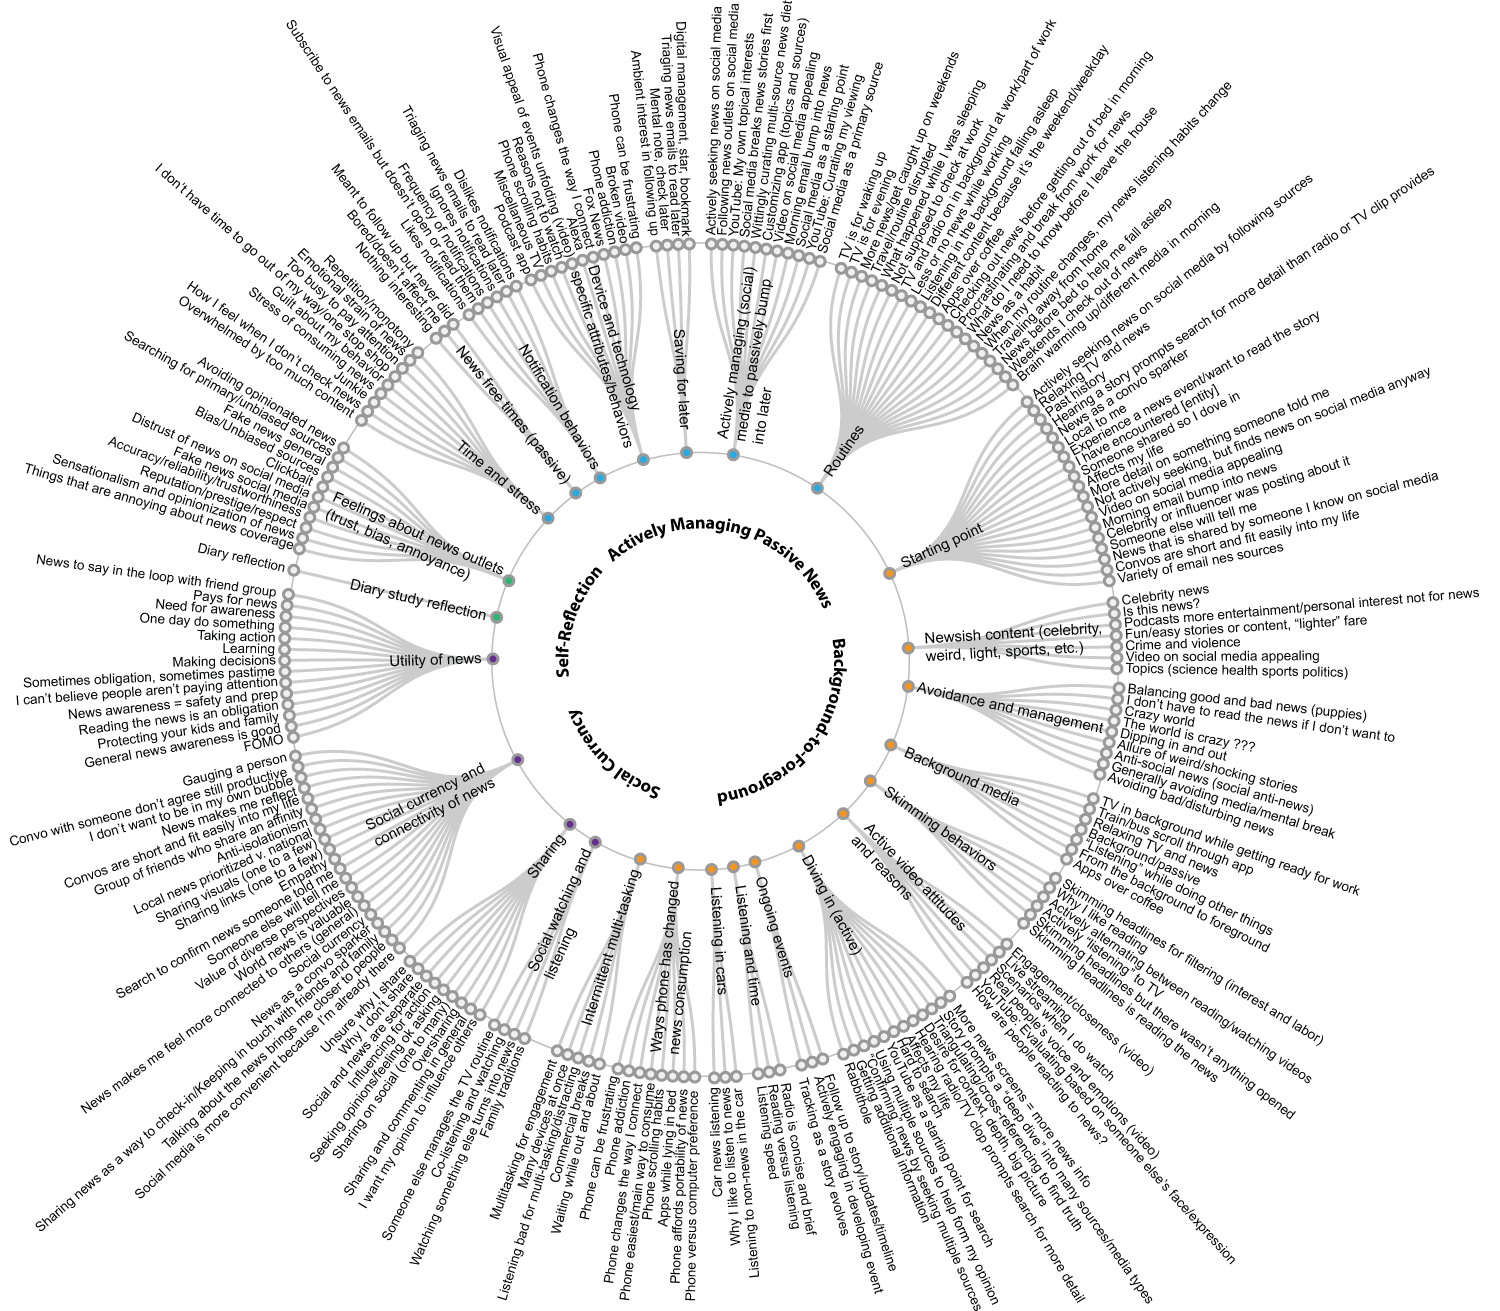
\includegraphics[width=\textwidth]{figures/circular-dengrogram.png}
  \label{fig:category-labels}
\end{figure*}

\subsection{Analysis}
Our analysis approach was inductive and anchored in the participants’ narratives of their own news behaviors. We first transcribed the pre- and post-study interviews and daily voicemails. We then did a close reading of these to identify rough themes, followed by a second reading to pull out direct quotes, behaviors and researcher observations that represented distinct ideas. This close reading resulted in 1100 notes, which represent our smallest unit of analysis. We then conducted an inductive analysis of those notes using an affinity diagramming technique, which both researchers iterated on collaboratively until we reached a consensus. Through affinity diagramming, we produced a hierarchical database: the notes were organized into 200 categories, which include a group of tightly-related notes; those categories were organized into 24 meta-categories, which include a group of tightly-related categories. The full codebook is available in our supplementary materials.

\section{Findings}
In this section, we will explore cross-media and cross-platform news behavior through four major themes: (1) news as a background-to-foreground activity, (2) news management strategies, including actively managing background news streams and time-shifting, (3) the social currency of news, and (4) the consequences of self-reflection. Figure \ref{fig:category-labels} visualizes how the meta-categories and categories from our affinity analysis fit into these themes.

\subsection{News as a background-to-foreground activity}
Checking in with news is often a passive, background activity, such as having the TV on in the background while getting ready for work in the morning, scrolling through Instagram while in line at the grocery store, or listening to the radio in the car. Participants described background news behaviors as routine and low-engagement, often combined with skimming and multitasking: 

\begin{quote}
    If I’m tending to skim only the headlines, I’m kind of in the middle of something else or kind of procrastinating. I don’t have, I guess, the energy capacity, necessarily, to go and click through every article. - SK, post-interview
\end{quote}

However, when a news story grabbed participants’ attention, their behavior became active: 
\begin{quote}
I’ll passively go through the news, I’ll passively listen to people have a conversation about topics that might be interesting. If something catches my ear I’ll listen more actively. - JW, post-interview
\end{quote}
This background-to-foreground behavior evokes the \textit{cocktail party effect} \cite{arons1992review}: Imagine yourself in a crowded room. Most of the conversations are unintelligible background noise. But when something catches your attention, like you hear your name, you are able to tune in to that conversation and tune out all other noise. At any time you can leave that conversation and tune into a different one or return to a soft focus on the background chatter. We observed something similar happening with news attention as participants shifted from background news consumption to foreground activities and back again. We’ve annotated the following quotes to illustrate background-to-foreground behavior—[B] indicates background news activities (the chatter), [F] indicates foreground activities (the focused attention), and [I] indicates inciting factors (the moment where you hear your name):
\begin{quote}
Wow, it was a pretty crazy day, but news circulated around one ... Well, two major stories, but one kicked off the day: Facebook, largest drop in the history of any stock, in terms of market cap. Instantly, \textbf{\textit{opened Yahoo, because earnings report was released. I was sitting at my desk about 8:15, 8:30 this morning reading articles. [B]}} So, the \textbf{\textit{drop in market value that Facebook had, was larger than McDonald’s entire market value [I]}}, itself. [...] Didn’t have too much time on my phone today. I saw some updates coming through, but I didn’t really pay attention to them today. They just kind of sat there. But, reading Yahoo articles while at work, \textbf{\textit{something I’m really interested in, because that’s my job, I work in finance [I]}}, and \textit{\textbf{watching CNBC [B]}},\textbf{\textit{ turning it up [F]}}. \textbf{\textit{It’s usually on mute [B]}}, but \textit{\textbf{we were turning up the volume [F]}} when it was \textit{\textbf{a story that we were a little bit more interested in [I]}}, and \textbf{\textit{we shared and discussed the story that we heard throughout the day [F]}}. So, it was a pretty wild day today at work. - BW, voicemail
\end{quote}
In this example, the participant’s background activities are routine news scanning while checking email and muted TV at work. Foreground activities are remembering key facts, turning the TV volume up, and actively discussing and sharing information with co-workers. The inciting factor is that the story that was relevant to the participant's job. During this active news event, other information faded into the background as the participant barely noticed other news alerts.

Any type of media can take a background or foreground role, and this plays out differently for reading, listening, and watching. Skimming notifications or headlines on a mobile phone, listening to the radio in the car, and having the TV on in the background while getting ready for work are all background activities. Reading multiple articles on a topic from different sources, selecting a favorite podcast to listen to on the bus, and searching for videos on YouTube are all foreground activities. 

We've summarized some of the background behaviors, foreground behaviors, and inciting factors we observed during the diary study in Table \ref{tab:backgroundforeground}.

\begin{table*}
  \caption{Examples of background-to-foreground news behaviors observed during the diary study}
  \label{tab:backgroundforeground}
  \begin{tabular}{p{5.5cm}p{5cm}p{5cm}}
    \toprule
    Background Behaviors [B]&Inciting Factors [I]&Foreground Behaviors [F]\\
    \midrule
    \ Scanning headlines while checking e-mail&Evokes personal memory or experience&Searching for more info on a topic\\
    \ Checking trending topics on Twitter&Know a friend would be interested&Seeking reactions from influencers\\
    \ TV on in the background while cooking&Story is alarming or surprising&Sharing a screen grab in a group text\\
    \ Casual chat with co-workers&Contains information for survival&Making a mental note to follow-up\\
    \ Scrolling through news app&Affinity for/special interest in a topic&Asking questions to family members\\
    \ Listening to radio while driving&Shared by close friend&Drawing connections to past events\\
\end{tabular}
\end{table*}

\subsection{Managing strategies for fitting news into daily life}
Whether our participants viewed news as an obligation or a hobby, they all experienced challenges fitting news consumption into their daily lives. Our participants managed their news consumption by developing strategies to: set themselves up to bump into personally relevant news; save content for later when they can not devote attention to the news; and transition back into the news after a deliberate or accidental break.

Although background news consumption is often passive, people actively curated their passive news streams to facilitate future foreground news experiences. Participants accomplished this by curating social media feeds by following news organizations or news-conscious friends, maintaining communication with social circles via group texts, installing and customizing mobile apps, managing app notification settings, and curating daily routines that facilitate background radio and TV consumption. Across all of these strategies, participants valued convenience, relevance, and the ease of fitting news into daily life. One participant turns to a customized news app because, "I only get what I wanted to read. So, it will be fast, it will be interesting to me." (IL, post-interview) Another participant uses LinkedIn app as her preferred background news source because:
\begin{quote}
It's easy to scroll through quickly when you have a moment. [...] So you want people to think like you but you also want more people that maybe don't think like you to give you more insight[...] My feed has become more interesting, I think. Like I've been getting more relevant material to me, at least lately, as I've added my network.  - CM, post-interview\end{quote}

In each of these examples, participants value the ability to find foreground stories that resonate. But people also curate background routines that keep them generally caught up with news, "I turned on the news, the NBC local news while waiting for my TV shows to watch and my spouse to get home." (LV, voicemail) In some cases, multi-tasking or multi-screening facilitated a faster switch between the background and the foreground. One participant who frequently searched on a phone for more context while watching TV news built this into a routine, "This is my TV, my desk, the laptop, and then usually I have two phones right here. This is just how I do the news sometimes." (MR, post-interview)

It’s quite common for people to disengage from the news: Every single participant had at least one voicemail acknowledging that news had played a diminished or nonexistent role in their lives that day. People disengage from news because they are busy, “Today was a super busy day, so I didn’t see a lot of news,” (SB, voicemail) or traveling, “I usually look at more news, but I was out for most of the day” (ML, voicemail). Sometimes, they intentionally disengaged due to news fatigue,"After all the nastiness today in the news, I am just going to go and listen to my silly armchair podcast while getting ready for bed." (LV, voicemail)
 
Some participants welcomed news free days, “I just like not having to look at my phone all the time” (SK, post-Interview). However, several participants expressed that disengaging from the news can increase their stress, "You know when...you don't have access to news and then you kind of come back and then there's all these stories and all this stuff going on and you almost feel behind." (CM, post-interview) For others, a day or two without any news is totally fine, but “when I get to a week or more without knowing anything about the news, then I start to get a little stir crazy” (JS, post-interview).

When people were unintentionally disengaging from the news, like they were busy, they demonstrated strategies for time-shifting content so that they could return to it later. One strategy is making a mental note to check on a story later:
\begin{quote}
[Interviewer: Do you remember how you first encountered this story?] On Yahoo. And then later on, I was interested in it, so I went on my sports app [...] I went into the basketball, the NBA, and they had other articles on Lebron opening up a school there. - BW, post-interview
\end{quote}
However, this mental note strategy doesn't always work, resulting in a failed inciting factor, "I'll see something or hear something and it's like, ‘Oh, that's interesting’ and then I'll move on. And then I'll never get back to it." (JW, post-interview)

Participants also used digital notes, "You know on your Gmail you can put a star or whatever, I'll highlight the star if it's something I wanna come back to."

When people were disengaging from the news, they often relied on their social groups as a distinct strategy for maintaining a connection to important events:
\begin{quote}
If I had missed something really important, someone would have brought it to my attention. (DR, post-interview)
\end{quote}
\begin{quote}
If there was something super important to happen, I would find out about it or someone will tell me about it or I’d hear about it or see it. - SK, post-interview
\end{quote}

\subsection{Social currency of news}
Offline and online relationships play major roles in how people navigate, make sense of, and relate to the news. As one participant noted, “Most of the news things today were conversations,” (SB, voicemail). Our diary study revealed insights about the way technology mediates group news engagement, the role of family traditions and social contexts in encountering background news, and the social incentives for news engagement.

Family, friends and co-workers served as de facto background news streams and as inciting factors, helping people stay in touch with current events and also inspiring them to dig in deeper to relevant stories. Many participants are involved in ongoing group or one-to-one text message chains where news intermingles with other types of content. In these social contexts, news isn’t simply information—it’s also a nudge to stay in touch:
\begin{quote}
Anything interesting, or funny, or even something stupid, we always just screenshot or somebody posted the link [...] there's like six of us in the group, and people like it or people start talking about it. - SA, pre-Interview
\end{quote}
News provides a shared vocabulary for real-time interaction, mediated by the immediacy of text messaging:
\begin{quote}
We're texting again about just everything that's unfolding [...] texting, even with my best friends, I feel like texting has taken over because sometimes we're all tired, work, and whatever, texting is just such an easy way to always be in touch with somebody in real time. - ML, post-interview
\end{quote}
Participants experienced news socially through co-listening and co-watching. This could be ad hoc, like the participant who listened to NPR because her Lyft driver was listening to it (LV, voicemail). Or it could be a codified family tradition:
\begin{quote}
  When I went to my grandmother's house, when I went to my aunt's house, we all watched the news. I can remember as way back as since I was young, 10 o’clock news come on, after the news come on channel 11, the Honeymooners used to come on with Jackie Gleecer. So I guess that's how I was raised watching the news. - CW, post-interview 
\end{quote}

The laddering questions using in the post-interview revealed potent social motivations for interacting with the news. Some participants got satisfaction from sharing news because it solidified relationships, "I like knowing I've introduced people to something maybe they haven't seen yet or that will be impactful for them or that they'll really enjoy." (LV, post-interview) Sharing might result in friends returning the favor, "It's kinda cool to sometimes just be the one to almost break a story to somebody...it’s kind of like a pay it forward type of thing." (BW, post-interview) News also serves as a connective tissue that helps people feel close to friends and family:
\begin{quote}
I think news to me, it's almost like you can say Sunday dinner, it brings me closer to my friends. - ML, post-interview
\end{quote}
\begin{quote}
I don't get to socialize a lot in my real life….So this is sort of how I socialize is sharing information back and forth and talking about the stuff we read and watch.  - LV, post-interview
\end{quote}
People saw conversations about the news as valuable elements of the news ecosystem that helped them make sense of events as well as connect with peers:
\begin{quote}
...even if they don't agree with you by the end of the conversation, they can go away, take away that they had a good view, a good back and forth with someone of a different view. - MR, post-Interview
\end{quote}
Being able to connect with peers about the news is so highly valued that several people expressed a fear of missing out:
\begin{quote}
“[I] don't want to be left out when my coworkers are talking about things so I usually try to kind of catch up on, try to see what they're talking about.” - IL, post-interview
\end{quote}
\begin{quote}
I don’t wanna go somewhere and there was a huge news story that everybody's talking about and I just have no clue what they're talking about, I can't engage and I'm just sitting there. - BW, post-interview
\end{quote}
For some, the ability to connect with people using news as a social currency was a primary driver for consuming news,
\begin{quote}
I just want to be kept in the loop. If I don't interact with the news, then I don't know what's going on in the world and I just feel like an outsider. - AB, post-interview
\end{quote}
News also helped people feel less isolated. One participant added hashtags to his Tumblr diary, unprompted. When we asked why, he said it helped him feel more connected: 
\begin{quote}
I feel like I was doing this in isolation, but to really see like okay, well when I put these hashtags and things are popping up [...] So to see that other people are consuming the news similarly to me, or that some of these same hashtags are trending, it tells me like okay, well what I'm following other people, there's interest in that as well. - ML, post-interview
\end{quote}
Paying attention to the news helped people feel connected to the broader world:
\begin{quote}
Yeah, it's probably pretty easy to get stuck in your own space, in your own bubble. But finding out the things happening in the world, it feels less like, I'm just living in a bubble, and more of just... I'm not necessarily experiencing all those things, but knowing about them and having views about them and can empathize with people. - SK, post-interview
\end{quote}

\subsection{Self-reflection about news behaviors}
Attrition is typical with diary studies of this length, so we were surprised to find that all 14 participants who began the study successfully completed it. Several participants said they enjoyed the study, "It was really fun...It was just so exciting...I really, really got into the experience." (CW, post-interview) Participating in the study provided people an opportunity to reflect and discover unexpected insights about their own news behaviors:
\begin{quote}
...having the right information from the right source is important to me, but I realized I wasn’t doing that. -DR, post-interview\end{quote}
\begin{quote}
Made me more aware of the news as it was coming to me as opposed to just being ‘ok whatever’ -JW, post-interview\end{quote}
\begin{quote}
[I thought news was] passive because I was doing it to kill time, but never until I did this realized how it was active - LV, post-interview\end{quote}

In some cases, participants wanted to modify their news behavior to align with their goals, either to engage with the news more—"I’ve learned that I skim too much through stories," (AB, post-interview)—or less—"I was quite surprised that I really do spend way too much time on my news apps. Need to put down the phone sometimes and read a book." (LV, post-interview)

Tracking personal news habits helped one participant see previously invisible connections between events, "I never realized until doing this that a lot of these stories compliment each other"—logging his  behaviors helped him see the "tapestry" of the news. (ML, post-interview)

\section{Limitations}
During a diary study, participants are aware they are being observed, which can cause them to change their behavior. The length of our study and our instructions to participants mitigated this observation effect. For example, one participant noted that for the first few days she felt like she was doing homework, and was researching news items in more depth than she normally would (JW, post-interview). After a few days, she remembered that she’d been instructed to just be normal, and returned to her normal news behavior.

By design, our research approach lacks clear boundaries. Once we allowed people to wander beyond the bounds of a single behavioral mode, media type, or platform, we couldn't be sure where they would go. We saw this in our diary study when participants questioned, “Is this thing news?” We tempered this ambiguity by reassuring participants that news content and platforms could be whatever fit their own personal definitions.

While our study size (n=14) is typical for a diary study, we had some demographic limitations. Participants were self-selecting in that we pulled them from a database of people who have signed up to participate in user research. Our participants were distributed across the U.S. and their habits covered a broad spectrum of political perspectives and topics—FoxNews, the BBC, indie news organizations; entertainment, politics, gaming. However, they were concentrated in urban areas (Bay Area, Houston, Chicago, New York) so this study doesn't include rural news consumers.

\section{Discussion}
In this section we discuss  how the limitations of a cross-platform approach led us to a more encompassing transmodal framework, which we define and demonstrate. Then we discuss how a transmodal approach is useful within HCI for understanding news and other behaviors. Finally, we present design implications for news products that draw on our diary study findings and recognize transmodal news behavior. 
\subsection{From cross-platform to transmodal research}
We began this study looking for differences in news consumption based on reading, listening, and watching behaviors. However, we found it impossible to talk to users about crossing media boundaries without talking about how they experience other boundary crossings as well. In our analysis, we iterated on different ways to define, describe, and characterize news behaviors. As a result, we shifted our focus beyond media types—text, audio, video—to consider the platforms and devices on which users accessed them—TVs, car radios, mobile news apps, Twitter. Platforms don’t exist in isolation, but are scaffolded by trellises that structurally support them and ladders that connect them to other features in the environment. Users don’t magically appear on platforms—they travel through this understudied scaffolding. To describe these traversals, we sought a frame that was more encompassing than cross-media or cross-platform behavior. We settled on the term \textbf{transmodal}\textit{}. Our approach to studying transmodal news behavior considers \textbf{how and why users switch between behavior modes, media types, platforms, devices and sources} (Table~\ref{tab:transmodal}). The term transmodal has connotations in supply-chain logistics, where it refers to goods that are shipped using multiple modes of transportation, and psychology, where it refers to multiple sensory and cognitive processes, but hasn't been widely used in HCI. The transportation connotation is fitting because a transmodal approach attends to the \textbf{\textit{transitions}} between different types of news experiences.

Drawing on the theory of uses and gratification, people manage their foreground and background news activities based on a range of contexts and goals. But these structural approaches don’t account for the limitations and affordances of the media cycle and the availability of media in different contexts. In any given moment, a person’s news consumption behaviors are mediated by goals (being bored and needing to pass the time, experiencing the fear of missing out, encountering a story that evokes a strong sense of nostalgia) and by locational and situational context (at home lounging in bed, out and about shopping, cooking dinner). These, in turn, influence the type of media they will seek out (easily digestible headlines, YouTube video showing influencer reactions, in-depth long-form story) and the device they’ll consume on (laptop, mobile phone, background TV). Further, personal preferences and social motivating factors influence how a person seeks information (searching, texting a friend with a question, going to a habitual news source) and the platforms they use. Using transmodality as a lens, we can bridge exclusively social nature of "uses and gratification" and the technologically deterministic nature of single-platform approaches to come up with a more useful socio-technical stance for understanding news media behavior. A transmodal approach leverages many different behavioral, material and contextual elements and focuses on the transitions between individuals, societal, and technological influences on users' behavior as a framework for evaluating news consumption experiences in HCI. 

\begin{table*}
  \caption{Elements of transmodal news behavior}
  \label{tab:transmodal}
  \begin{tabular}{ll0}
    \toprule
    Element&Key questions&Examples\\
    \midrule
    \ Activity Mode&What is the user doing?& reading, listening, watching\\
    \ Media&What is the user consuming?&text, audio, video\\
    \ Platform/Device&How is it being distributed?&news app, Facebook, car radio, TV\\
    \ Source&Where does it come from?&New York Times, primary source, co-worker\\
  \bottomrule
  \ \textbf{Transmodal News Behavior}&\textbf{How/why is the user engaging?}&\textbf{Searching on phone for more context}\\
  \ \textbf{and Transitions}&\textbf{Why is the user switching experiences?}&\textbf{about a TV news story}\\
\end{tabular}
\end{table*}

\subsection{Analyzing transitions in news behavior}
How does a transmodal approach help us understand news consumption experiences? Let's take the example of a person listening to public radio news in the car on the way to work. She hears a story that catches her attention about an earthquake that triggered a tsunami near her hometown. When she gets to work, she searches for more information about that story on Twitter. Using a transmodal approach, we can map out the elements of this behavior: In the car, she is listening (behavioral mode) to audio (media type) on a car radio (platform/device) from NPR (source); at work, she transitions to reading and watching (behavioral modes) text and video (media types) on the mobile Twitter app (platform/device) from emergency management services, eye-witnesses, and individual journalists (sources). A transmodal approach encourages us to ask, What values and motivations drove her to switch between these news experiences? Perhaps the transition was motivated by an inability to devote full attention to the news story while in the car, or a desire to find additional information, or an urge to share this news with a friend. These transitions, and their motivators, open up new lines of inquiry that we would have not encountered had we simply studied radio listening habits or phone use logs. 

In our study, a transmodal approach helped us think about people's behaviors in new ways and surfaced unexpected insights, like the social currency of news we identified in the findings section. A transmodal framing opens up new lines of research into news and media consumption behaviors: Are certain elements of transmodality more dominant in driving people's news decisions? If we map a person's news habits onto a transmodal space, do people tend to stay in sub-regions of this space during different types of day or for accessing certain types of content? Looking at news behavior in this way lets us identify areas where people's goals and motivations for consuming news may be misaligned with their behavior patterns, which allows us to design better news experiences.

To fit into a broader set of methods for understanding user experiences, a transmodal approach should be coupled with approaches that can offer structure and definition. For example, researchers could pair transmodal studies with quantitative platform-specific log analysis to see if patterns observed play out. Or, researchers could collapse a transmodal view into a single platform, device, media type, or behavioral mode to observe that constrained environment before zooming back out to a transmodal perspective. A transmodal research approach, paired with an appropriate set of complementary methods, allows us to perceive users through the social and technological scaffolds that brought them to a given platform or media type to more deeply understand their information needs. This approach might be useful in understanding how to design for emerging technologies, like voice interfaces, so that they fit seamlessly into people's lives. Or it might help us learn how mis- and disinformation spreads, and how to build trust and verification into information ecosystems.

\subsection{Design to support intentional and unintentional news management behaviors}
We observed that people employed a range of intentional and unintentional strategies to manage the emotional and mental labor of keeping up to date with the news. To meet the needs of users, designers can incorporate features that support these management strategies.

\textit{Intentional strategies} include curating background news sources, building routines, and saving content for later. News product designs can facilitate these strategies by making it easy for users to customize ambient background news flows, both in content and form, to increase the chances of inciting moments. Content could be designed to fit into different routines with briefs and deep-dives. Active foreground behaviors such searching, synthesizing, and finding reactions to news events should be supported. Users should be able to easily save content for later, across platforms and sources, but should also be able to give themselves a clean slate so that the news doesn't become overwhelming.

\textit{Unintentional strategies} include treating news as a background activity and taking breaks from the news. Background news consumption habits such as skimming and multi-screening are sometimes seen as peripheral to news engagement. However, our study revealed that background news consumption is a critical part of a healthy news diet—it's the fiber that keeps the system running smoothly. News product design should facilitate, rather than resist, background behaviors by treating them as mandatory steps in the ladder of news engagement. This could include presenting content in a way that affords for quick skimming behavior and making diving-in points explicit and easy to access. News apps should welcome users back from breaks with the most relevant information.

\subsection{Design to support extrinsic and intrinsic motivations for news consumption}
People experienced extrinsic rewards for keeping up with the news, such as enhanced social connectivity, as well as intrinsic rewards, such as feeling informed and prepared. These extrinsic and intrinsic rewards suggest design implications.

\textit{Extrinsic motivations} included being able to connect and converse with strangers, friends and co-workers. People sustain multi-directional news flow through activities such as group texts and in-person conversations. News products could give users the ability to quickly get caught up with major news, ensuring they can get an overview of events and talking points to facilitate social interaction around that topic. One-to-one and one-to-few sharing should be seamless. Other design features include highlighting what's trending in local areas and what people who share an affinity are paying attention to. Discussion is an important avenue for people to process and interpret news, so we encourage news outlets to push themselves to provide meaningful ways for people to ask questions about the news.

\textit{Intrinsic motivations} included the self-reflection produced by engaging with the news. Our participants enjoyed how the diary study because it allowed them to learn more about their own news habits and, in some cases, motivated them to change their behavior. For example, one participant noted that the study, "was fun. It got me more involved with the news more than it did before. Because before, I mean, I looked, and then I walked away from it." (SA, post-interview) In HCI, we typically associate self-tracking with physical fitness and wellness, but our study showed that self-tracking has potential to engage people with news and to help maintain healthy news and information habits. News product designers could leverage this by showing users a list of the topics they most frequently click on, or the types of stories with which they spend the most time. Users already sense that their news habits are implicitly reflected in customization algorithms, but we observed that people have a desire to see this information explicitly so that they can act on it.

Framing news as a background-to-foreground activity makes us question the prevailing metrics news organizations use to evaluate engagement—can we imagine new metrics beyond page views, impressions, shares and likes? We encourage news product teams to look for metrics that can more accurately capture the engagement of a T-shaped user, perhaps by measuring the ratio of a user's background to foreground time, or the number and diversity of sources and activities a user engages with during foreground events. These new metrics could be appealing to users and be useful to news organizations.

\section{Conclusion}
News users access and process information in complex social and technological contexts. To understand the holistic environments in which people engage with news across multiple behavioral modes, media types, technology platforms, devices, and sources, we conducted a two-week diary study with 14 participants. Our transmodal approach to studying news behavior revealed the importance of background news in managing the social and emotional labor of keeping up with the news, the role of news in maintaining social relationships, and the potential to tap into self-tracking behavior as a way to encourage well-rounded news habits. These contributions should help designers create news platforms that help news users take control of their own news habits and navigate the tumultuous news and information ecosystem. Further, a transmodal approach, which looks at a person’s holistic technology use, can be applied to many other domains within HCI to more deeply understand motivations and behaviors.


\section{Parking Lot of Deleted things}
Diary studies have several potential drawbacks: Ultimately, the participant decides what information is relevant, not the researcher; additionally, when people know they are being studied, their behavior often changes. We tailored our analysis methods to account for these features by using laddering questions to uncover the values underlying the meaningful interactions participants chose to document and using the observation affect as an opportunity to invite participants to reflect on their own news behaviors.


(From introduction of transmodal concept):
A person using YouTube as a news platform to search for contextual information that can help her decide how to process a news event may arrive there after receiving a text message from a family member and hearing snippets of coverage on the radio. These fragments of news exposure influence her reasons for accessing YouTube and the questions she has in her head when she arrives. To fully understand users’ needs once they’ve arrived at a platform, we need to understand why they set out on their journey, how they arrived, and where they are headed. 

(From instrinsic motivations/self-tracking):
The reflective power of self-tracking has implications for research as well product design: The observation effect can be a methodological feature rather than a flaw, as the awareness our diary study produced allowed us to see otherwise invisible behaviors and values. One participant expressed a desire to have an even closer interaction with the researcher by discussing stories as they unfolded rather than only at the end of the study (AB, post-interview). This opens up possibilities for discussion-based research that leverages self-awareness even more by closing the loop between researcher and participant.

However, the danger of an unbounded  transmodal approach is that if you are looking for everything, you might end up finding nothing.

(from intro outline)
[HERE WE INTRODUCE CROSS-MODAL STUFF WITHOUT ACTUALLY DEFINING IT]
What is the person \textit{doing}? - behavior mode --> behavior
What is the person consuming? --> media
What is the person consuming it on? --> device
How is it being distributed? Where do they get it --> platform
Where does it come from? --> cross-source

Term:        Defined:        Examples:
Cross Media   Format consumed   article, video, radio broadcast
Cross device    what consumed on    phone, tablet, car radio, speaker

there are many ways to do this. People can switch devices, platforms, etc...

discussion:
Lots of modalities. Here we outline and define them:
Table

Together, its clear that this is complex == transmodality

In this paper, we adopt the term \emph{transmodal news consumption} to discuss how complex the news experience is with users frequently switching between modes of behaviors, media types, platforms, and sources.

Understanding transmodal news behaviors is important because how news information reaches people influences how they receive and interpret it.

- Ability to quickly get caught up with major news stories in a brief and digestible way, ensuring individuals can get an overview of news events and talking points to facilitate social interaction. this is inline with the above section highlighting the importance of background and skimming behavior which users so clearly value. 
- ability to quickly share in 1:few groups such as messaging apps
- social media can provide opportunities to highlight trending stories, topics, and opinions around hard and soft news stories. Being able to see what's trending in local areas, or with people sharing affinities, may also increase the ability for people to discuss news events. 

\begin{figure*}
  \caption{How Qualitative Themes Emerged Through Pre-Interview, Diary, and Post-Interview Stages}
  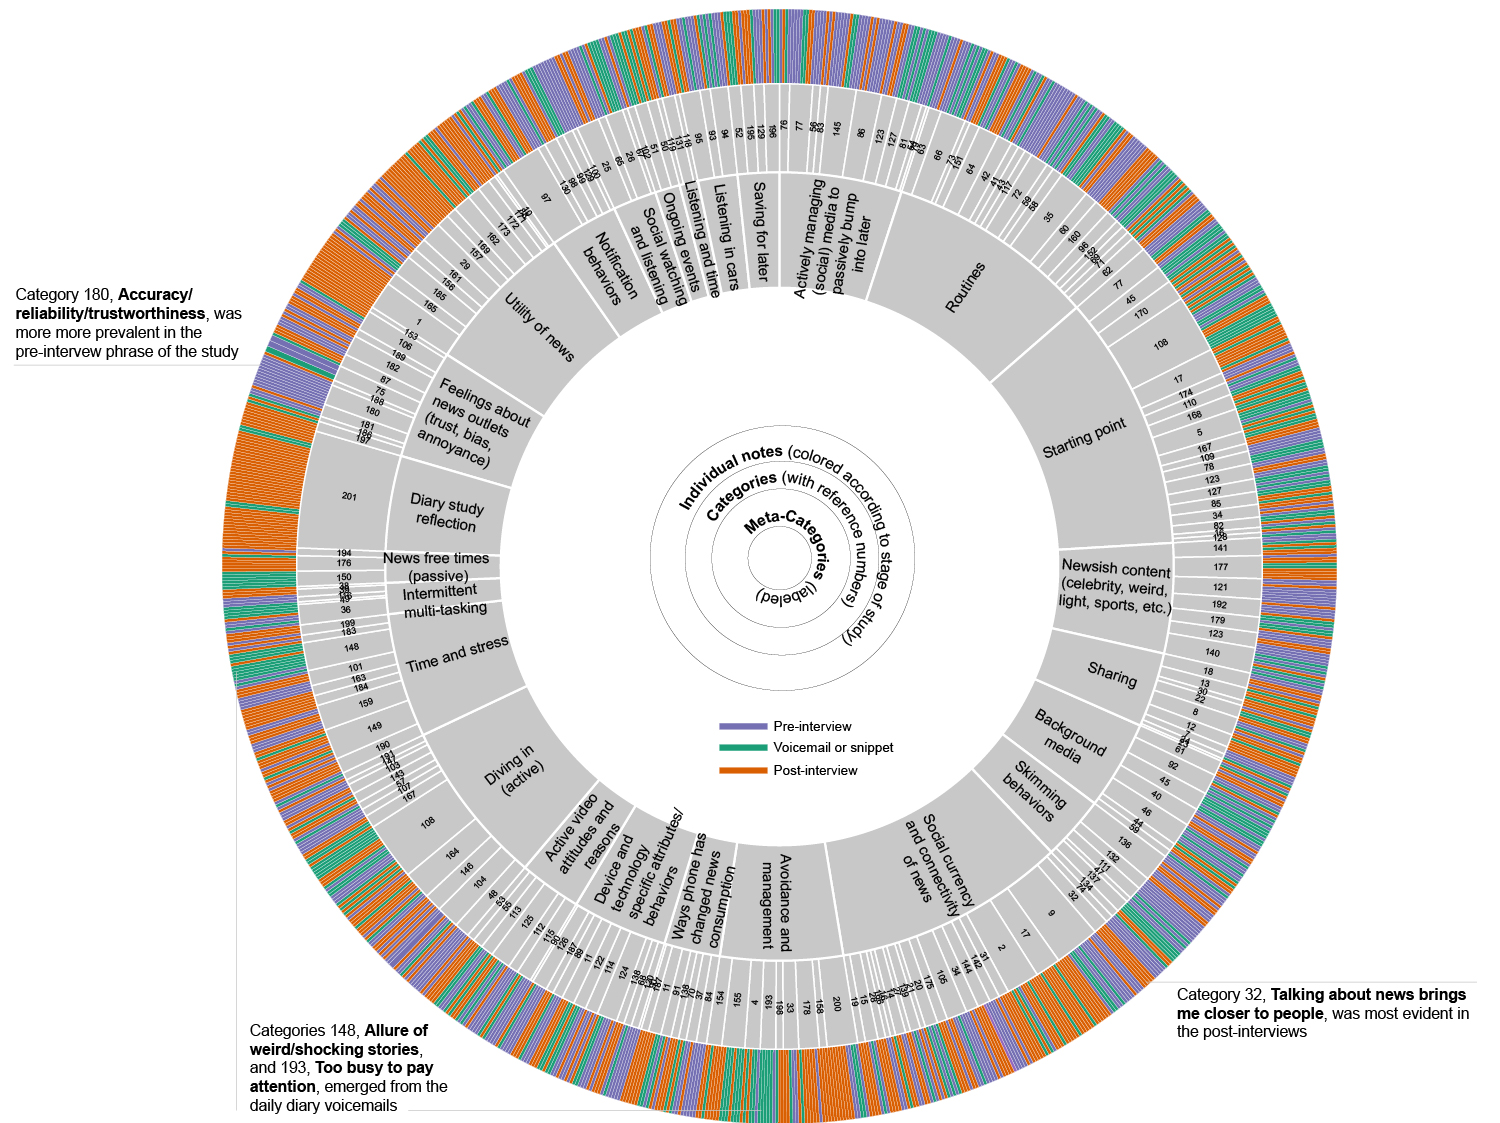
\includegraphics[width=\textwidth]{figures/circular-blocking-cleaned-nonsquare.jpg}
  \label{fig:codes-by-stage}
\end{figure*}

Here’s another example:
\begin{quote}
So, the first time I saw it I think it was on \textbf{\textit{AOL. That’s usually where I first see if any news is and unless I really search for news. [B]}} And I saw [Demi Lovato] was hospitalized for overdose and \textit{\textbf{I know about her history of being addicted to drugs [I]}}, that she was trying to come out clean. And she recently had a single out, a song out that she’s sober so \textit{\textbf{seeing that she’s still battling with a drug and everything I wanted to know like...what was pulling her back. [F]}} [...][I'm] \textit{\textbf{kinda a big fan of hers [I]}} so I \textit{\textbf{kept that in the back of my mind [F]}} and \textit{\textbf{on Instagram I think the next day [F] }}[...] the Jonas brothers are very close to her and they’re like next to her so they’re very close to her like a best friend...Basically yeah, that was \textit{\textbf{me seeing what they had to say anything about it. I went to their page, I scroll on Nick Jonas' page and Demi Lovato’s page to see any updates [F]}}, I didn’t see any. - DR, post-interview
\end{quote}
Here, the participant’s background activity is, again, habitual news scanning while checking email; her foreground activities are making active connections with other recent events, expressing curiosity by asking questions, making a mental note to follow up later, and checking Instagram to look for more information. The inciting factors are the participant’s affinity for Demi Lovato and her memory of past news events.

\begin{figure}
    \centering
     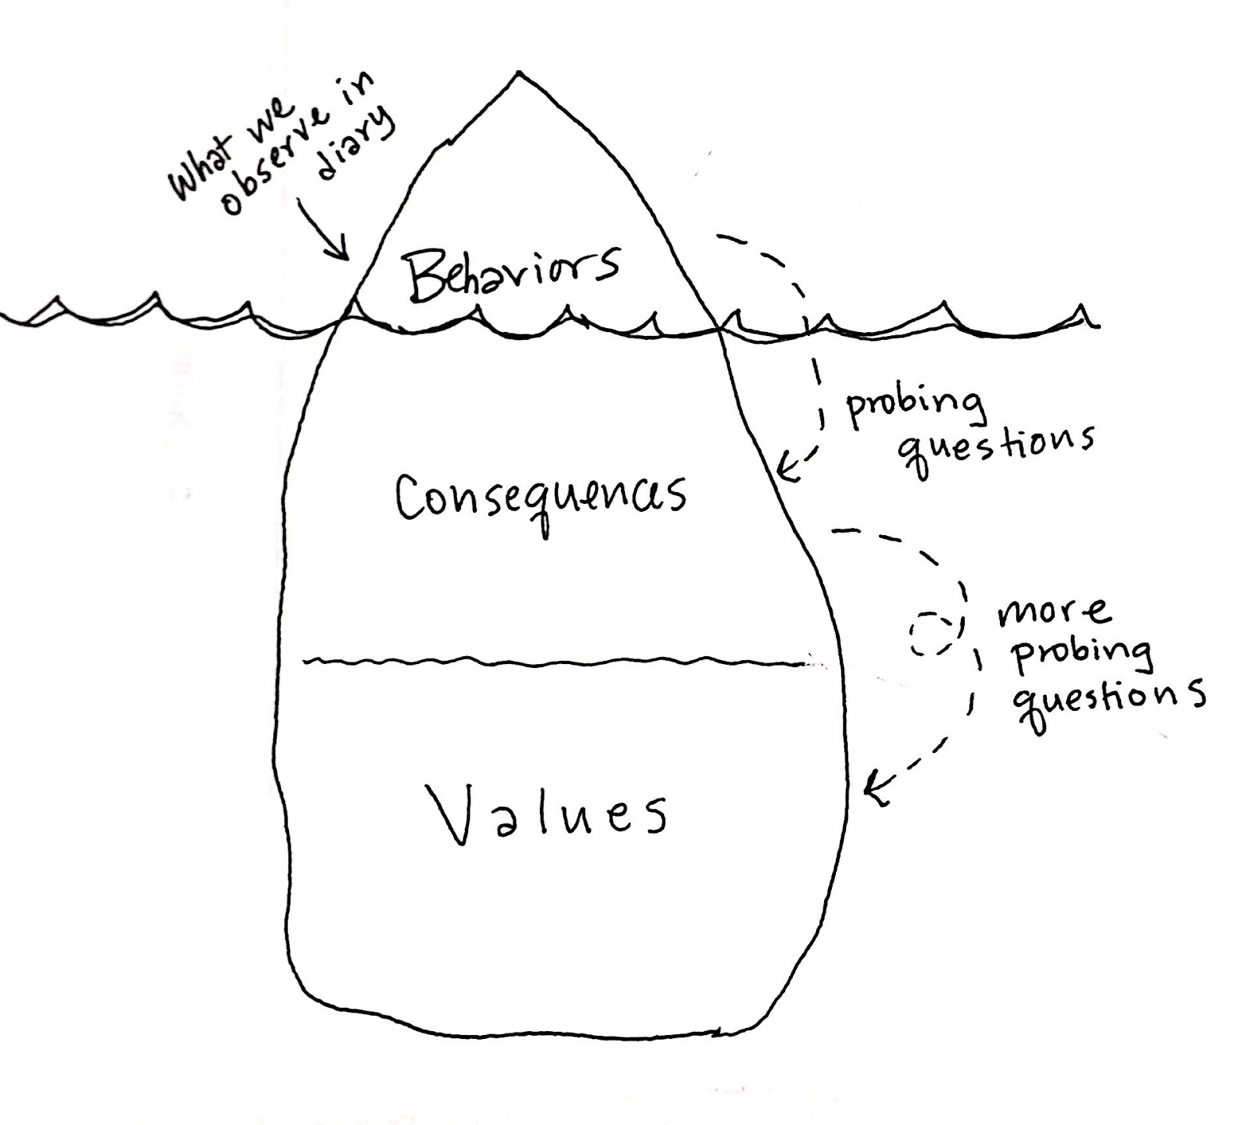
\includegraphics[width=\columnwidth]{figures/laddering.png}
    \caption{The laddering technique uses probing "why" questions to uncover the underlying consequences and values beneath observed behaviors}
    \label{fig:laddering}
\end{figure}


\begin{figure}
  \caption{People exhibited T-shaped news behavior, with background ambient news, inciting factors, and engaged foreground activity.}
  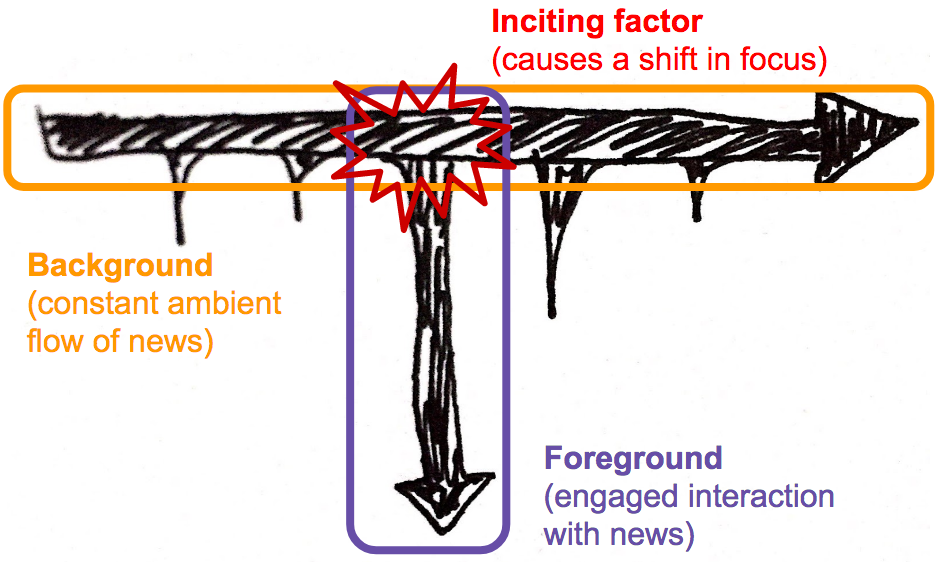
\includegraphics[width=\columnwidth]{figures/t-shaped-behavior.png}
  \label{fig:tshapedbehavior}
\end{figure}

Foreground engagement can be fairly shallow, like sending a text to a friend with a link or screen grab, mentioning a story to a co-worker in passing, making a mental note to follow-up, or adding a story to a digital queue. But it can also be deep engagement, like having a conversation with friends or co-workers, carrying out extended group or one-on-one text message exchanges, or searching to verify events, triangulate sources, find reactions, or get background context. Inciting factors cause a shift in focus from the background to the foreground. They can be social, like a friend or family members sharing news, or recognizing that it a story will be meaningful to a member of a close social group. They can also be personal, like having a history with or connection to a topic. If a story is surprising, delightful, or shocking, it can be inciting on its own.


This insight was only possible through a diary study: In the pre-interview, CM did not list LinkedIn as a regular news source. She wasn't conscious of how much she used it until she reflected on her own new behaviors, "During the study, a way that I found news during the study a lot, for some reason what LinkedIn news...maybe I was doing this more before and I just didn't even realize." (CM, post-interview) 

Others intentionally kept their sustained news level low, "If I always paid attention to the news, I’d be like chicken little thinking the sky is falling...and that’s just not how I chose to live my life." (JW, post-interview) 

\bibliographystyle{ACM-Reference-Format}
\bibliography{references}

\end{document}